% Adjust these for the path of the theme and its graphics, relative to this file
%\usepackage{beamerthemeFalmouthGamesAcademy}
\usepackage{../../beamerthemeFalmouthGamesAcademy}
\usepackage{multimedia}
\graphicspath{ {../../} }

% Default language for code listings
\lstset{language=C++,
        morekeywords={each,in,nullptr,int32, TCHAR, uint8, int8, uint16, int16,
        uint32, int32, uint64, int64, PTRINT, UObject. AActor, SWidget, FName,
        FString, UClass, USoundCue, UTexture}
}

% For strikethrough effect
\usepackage[normalem]{ulem}
\usepackage{wasysym}
\usepackage{listings}
\usepackage{pdfpages}

% http://www.texample.net/tikz/examples/state-machine/
\usetikzlibrary{arrows,automata}

\newcommand{\modulecode}{COMP260}\newcommand{\moduletitle}{Distributed Systems}\newcommand{\sessionnumber}{5}

\begin{document}
\title{\sessionnumber: 12}
\subtitle{\modulecode: \moduletitle}

\frame{\titlepage}

\begin{frame}
	\frametitle{Learning outcomes}
	\begin{itemize}
		\item \textbf{Identify} the various parts of the Arduino and their function
		\item \textbf{Explain} the difference between analog and digital
		\item \textbf{Implement} a basic interface using Arduino and openFrameworks
	\end{itemize}
\end{frame}


\begin{frame}
	\frametitle{What is an Arduino?}
	\begin{figure}
		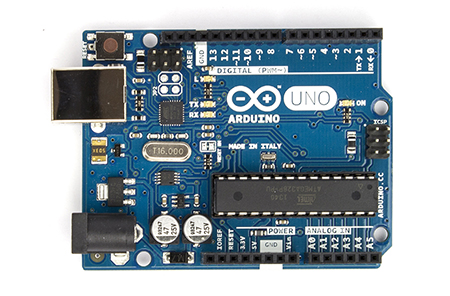
\includegraphics[scale=1.2]{assets/arduino}  
	\end{figure}
\end{frame}


\begin{frame}
	\frametitle{Sensors \& Actuators}
	\begin{figure}
		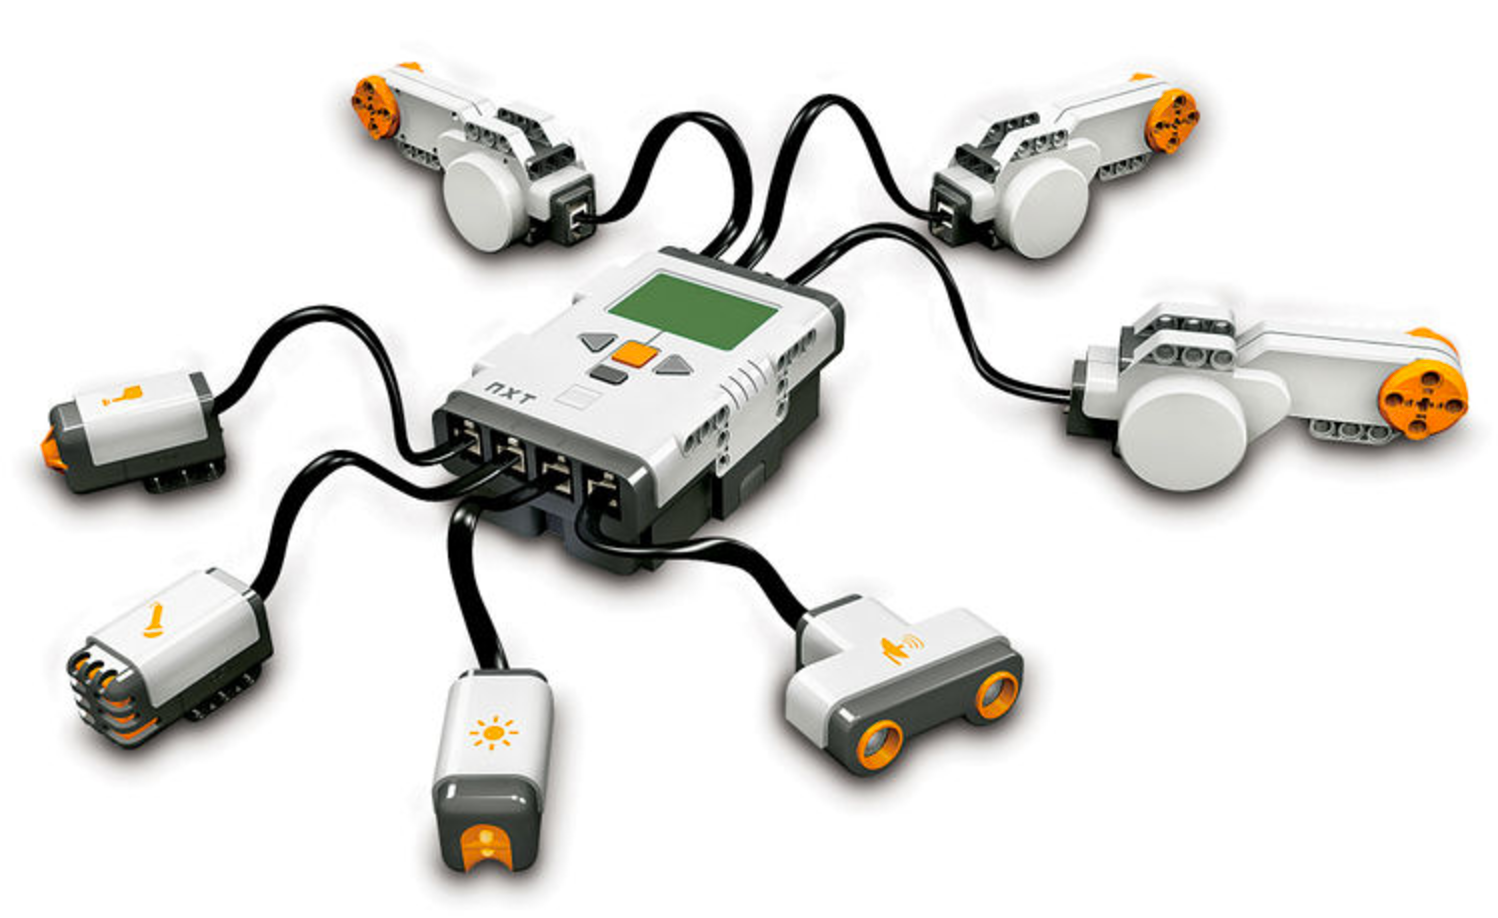
\includegraphics[scale=.15]{assets/nxt}  
		\caption{Just another input / output controller }
	\end{figure}
\end{frame}


\begin{frame}
  \frametitle{What is an Arduino?}
  \begin{itemize}
    \item Open Source
    \item The Arduino is a small microcontroller board
    \item Basically, a small computer 
    \item Perfect for rapid prototyping physical computing systems
    \item Arduino Uno is based on the Atmel ATmega328P
  \end{itemize}
\end{frame}



\begin{frame}
  \frametitle{The basics}  
  The Arduino can only prcesses electronic signals. This means that stimuli from the physical world need to be transduced to electrical signals before they can be processed from within your code. 
  
  \begin{itemize}
    \item 14 Digital IO pins (0-14)
    \item 6 Analogue in pins(0-5)
    \item 6 Analogue out pins(3,5,6,9,10, and 11) ~
  \end{itemize}
\end{frame}

\begin{frame}
	\frametitle{Technical specs}
	\begin{figure}
		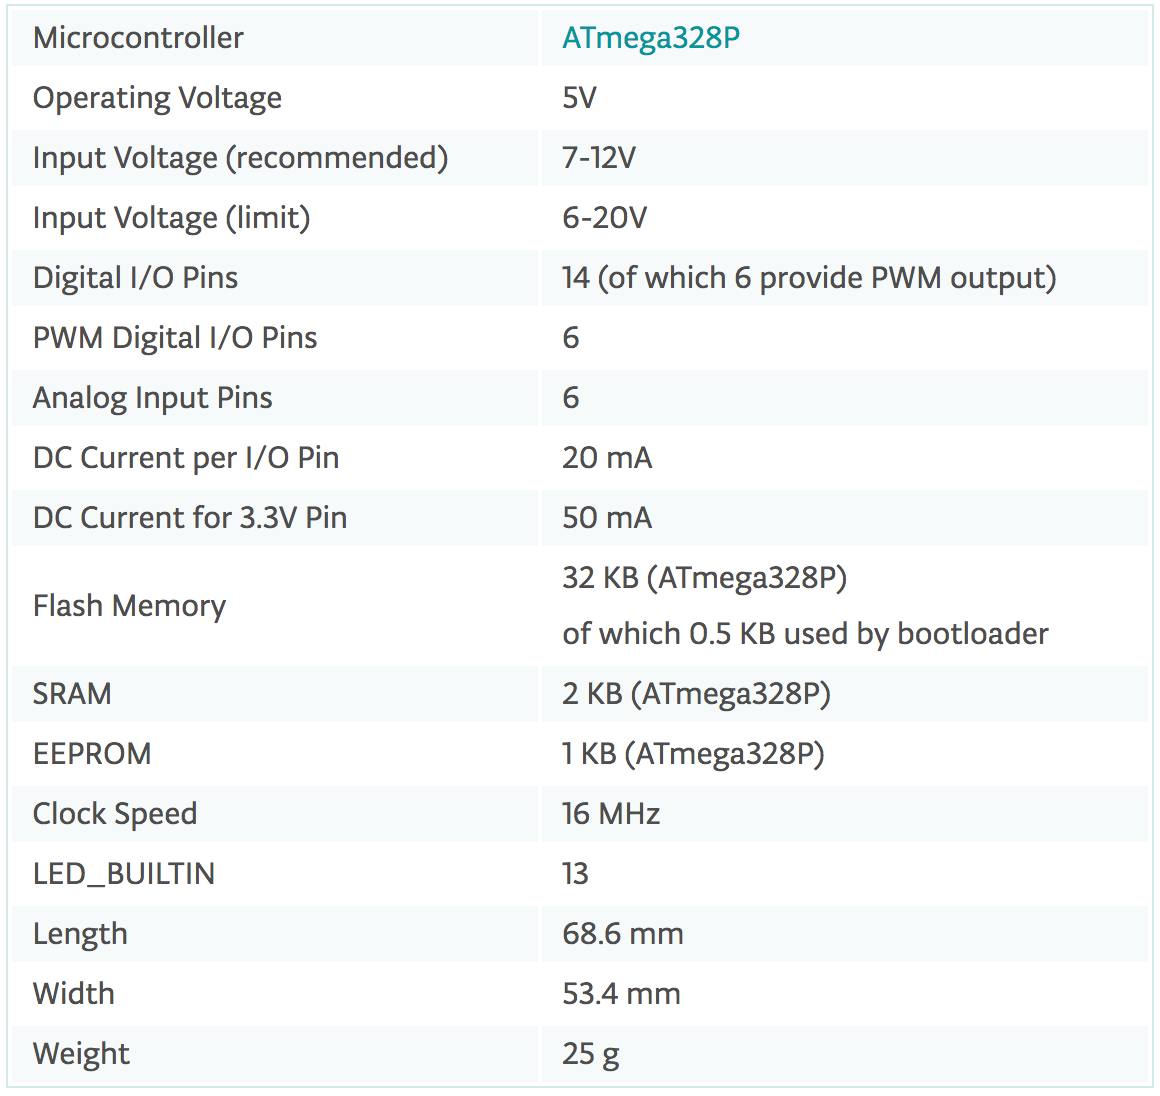
\includegraphics[scale=.14]{assets/spec} 
		\caption{A more in depth version of what the Arduino Uno has to offer}
	\end{figure}
\end{frame}

\begin{frame}
	\frametitle{Memory}
	\begin{itemize}
		\item Flash memory (program space), is where the Arduino sketch is stored.
		\item SRAM (static random access memory) is where the sketch creates and manipulates variables when it runs.
		\item EEPROM is memory space that programmers can use to store long-term information.	
	\end{itemize}
\end{frame}


\begin{frame}
  \frametitle{Power}
	You can power the board using a USB port or DC power supply such as a 9v battery. The Arduino will default to the external power supply if there is one available.   
	\begin{figure}
		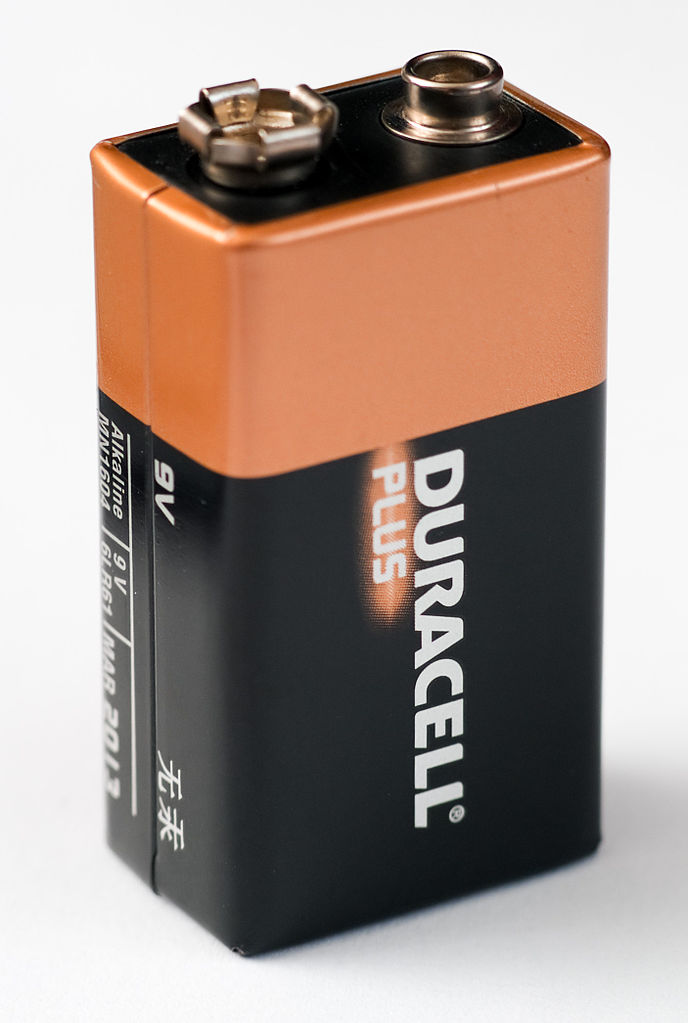
\includegraphics[scale=.1]{assets/battery} 
		\caption{Arduino can be powered by a DC supply 7-12v}
	\end{figure}
\end{frame}

\begin{frame}
	\frametitle{Analogue vs. Digital Signal}
	What is the difference? 
	
	\pause
	 \begin{figure}
		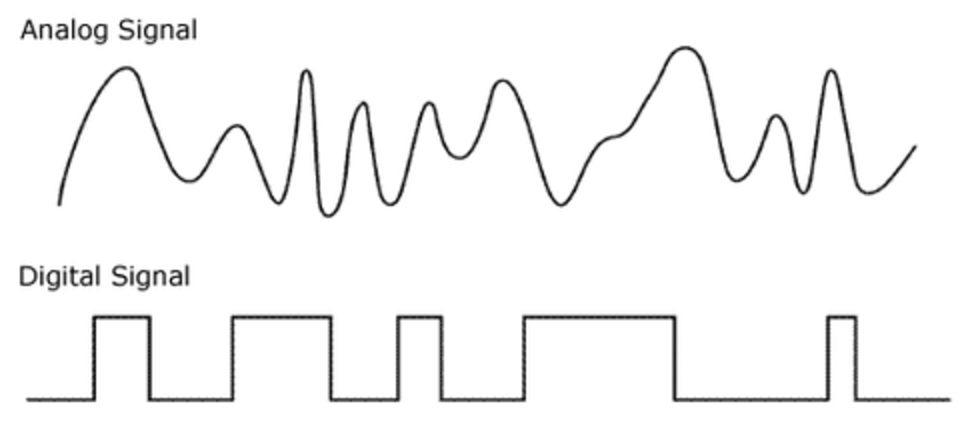
\includegraphics[scale=.3]{assets/dva} 
		\caption{Arduino can be powered by a DC supply 7-12v}

	\end{figure}
\end{frame}

\begin{frame}
 	\frametitle{Ohms Law - Comic}
   	\begin{figure}
   		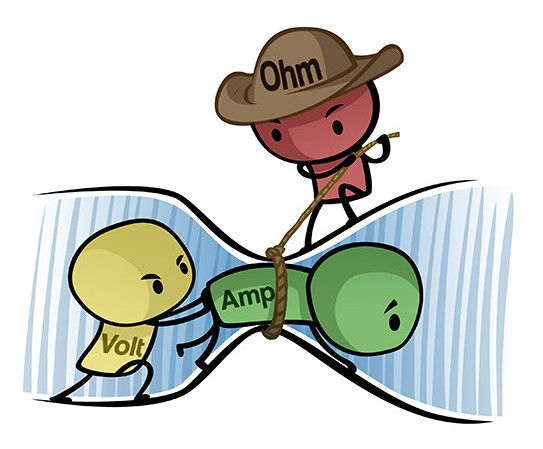
\includegraphics[scale=.3]{assets/ohm} 
	\end{figure}
\end{frame}

\begin{frame}
	\frametitle{Analogue Out - PWM}
	\begin{figure}
   		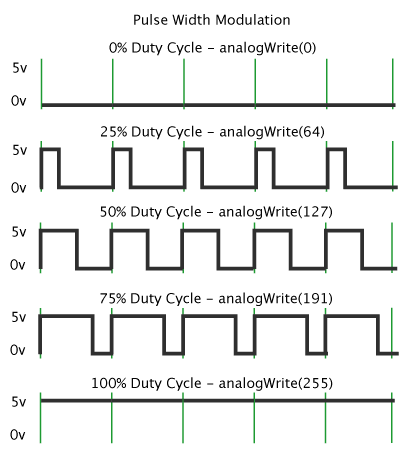
\includegraphics[scale=.4]{assets/pwm} 
	\end{figure}
\end{frame}

\begin{frame}
	\frametitle{Serial Communication}
	Serial communication on pins TX/RX uses TTL logic levels (5V or 3.3V depending on the board). \\~\\
		
	It communicates on digital pins 0 (RX) and 1 (TX) as well as with the computer via USB. Thus, if you use these functions, you cannot also use \\~\\pins 0 and 1 for digital input or output. 
	
	
	Serial is used for communication between the Arduino board and a computer or other devices. 
	
\end{frame}

\begin{frame}
	\frametitle{Driving Bigger Loads}
\end{frame}

\begin{frame}
	\frametitle{Breadboard}
	\begin{figure}
		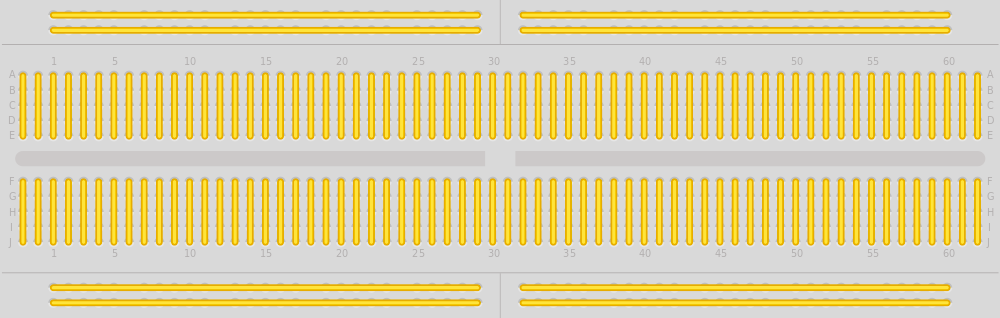
\includegraphics[scale=.25]{assets/breadboard} 
		\caption{The layout of the connectors inside the bread board}
	\end{figure}
\end{frame}

\begin{frame}
	\frametitle{Shields}
	\frametitle{Breadboard}
	\begin{figure}
		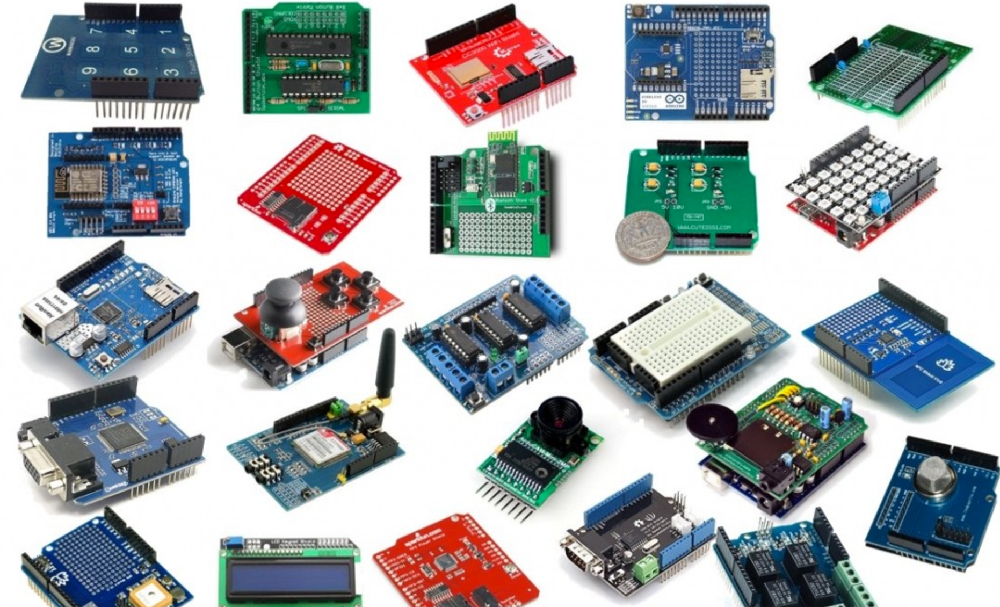
\includegraphics[scale=.28]{assets/shields} 
	\end{figure}
\end{frame}

\begin{frame}
	\frametitle{Open Source Game Boy Clone}
	\frametitle{Breadboard}
	\begin{figure}
		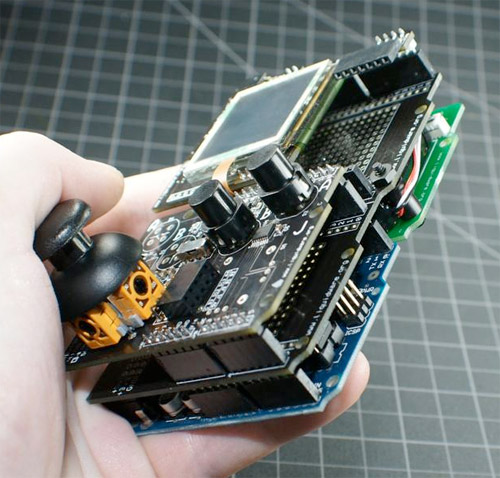
\includegraphics[scale=.32]{assets/gameboy} 
	\end{figure}
\end{frame}


\end{document}
